% Options for packages loaded elsewhere
\PassOptionsToPackage{unicode}{hyperref}
\PassOptionsToPackage{hyphens}{url}
%
\documentclass[
  english,
  doc,floatsintext]{apa6}
\usepackage{amsmath,amssymb}
\usepackage{lmodern}
\usepackage{ifxetex,ifluatex}
\ifnum 0\ifxetex 1\fi\ifluatex 1\fi=0 % if pdftex
  \usepackage[T1]{fontenc}
  \usepackage[utf8]{inputenc}
  \usepackage{textcomp} % provide euro and other symbols
\else % if luatex or xetex
  \usepackage{unicode-math}
  \defaultfontfeatures{Scale=MatchLowercase}
  \defaultfontfeatures[\rmfamily]{Ligatures=TeX,Scale=1}
\fi
% Use upquote if available, for straight quotes in verbatim environments
\IfFileExists{upquote.sty}{\usepackage{upquote}}{}
\IfFileExists{microtype.sty}{% use microtype if available
  \usepackage[]{microtype}
  \UseMicrotypeSet[protrusion]{basicmath} % disable protrusion for tt fonts
}{}
\makeatletter
\@ifundefined{KOMAClassName}{% if non-KOMA class
  \IfFileExists{parskip.sty}{%
    \usepackage{parskip}
  }{% else
    \setlength{\parindent}{0pt}
    \setlength{\parskip}{6pt plus 2pt minus 1pt}}
}{% if KOMA class
  \KOMAoptions{parskip=half}}
\makeatother
\usepackage{xcolor}
\IfFileExists{xurl.sty}{\usepackage{xurl}}{} % add URL line breaks if available
\IfFileExists{bookmark.sty}{\usepackage{bookmark}}{\usepackage{hyperref}}
\hypersetup{
  pdftitle={Early Biomarkers of Parkinson's Disease Based on Natural Connected Speech},
  pdfauthor={Anja Probst1},
  pdflang={en-EN},
  pdfkeywords={keywords},
  hidelinks,
  pdfcreator={LaTeX via pandoc}}
\urlstyle{same} % disable monospaced font for URLs
\usepackage{color}
\usepackage{fancyvrb}
\newcommand{\VerbBar}{|}
\newcommand{\VERB}{\Verb[commandchars=\\\{\}]}
\DefineVerbatimEnvironment{Highlighting}{Verbatim}{commandchars=\\\{\}}
% Add ',fontsize=\small' for more characters per line
\usepackage{framed}
\definecolor{shadecolor}{RGB}{248,248,248}
\newenvironment{Shaded}{\begin{snugshade}}{\end{snugshade}}
\newcommand{\AlertTok}[1]{\textcolor[rgb]{0.94,0.16,0.16}{#1}}
\newcommand{\AnnotationTok}[1]{\textcolor[rgb]{0.56,0.35,0.01}{\textbf{\textit{#1}}}}
\newcommand{\AttributeTok}[1]{\textcolor[rgb]{0.77,0.63,0.00}{#1}}
\newcommand{\BaseNTok}[1]{\textcolor[rgb]{0.00,0.00,0.81}{#1}}
\newcommand{\BuiltInTok}[1]{#1}
\newcommand{\CharTok}[1]{\textcolor[rgb]{0.31,0.60,0.02}{#1}}
\newcommand{\CommentTok}[1]{\textcolor[rgb]{0.56,0.35,0.01}{\textit{#1}}}
\newcommand{\CommentVarTok}[1]{\textcolor[rgb]{0.56,0.35,0.01}{\textbf{\textit{#1}}}}
\newcommand{\ConstantTok}[1]{\textcolor[rgb]{0.00,0.00,0.00}{#1}}
\newcommand{\ControlFlowTok}[1]{\textcolor[rgb]{0.13,0.29,0.53}{\textbf{#1}}}
\newcommand{\DataTypeTok}[1]{\textcolor[rgb]{0.13,0.29,0.53}{#1}}
\newcommand{\DecValTok}[1]{\textcolor[rgb]{0.00,0.00,0.81}{#1}}
\newcommand{\DocumentationTok}[1]{\textcolor[rgb]{0.56,0.35,0.01}{\textbf{\textit{#1}}}}
\newcommand{\ErrorTok}[1]{\textcolor[rgb]{0.64,0.00,0.00}{\textbf{#1}}}
\newcommand{\ExtensionTok}[1]{#1}
\newcommand{\FloatTok}[1]{\textcolor[rgb]{0.00,0.00,0.81}{#1}}
\newcommand{\FunctionTok}[1]{\textcolor[rgb]{0.00,0.00,0.00}{#1}}
\newcommand{\ImportTok}[1]{#1}
\newcommand{\InformationTok}[1]{\textcolor[rgb]{0.56,0.35,0.01}{\textbf{\textit{#1}}}}
\newcommand{\KeywordTok}[1]{\textcolor[rgb]{0.13,0.29,0.53}{\textbf{#1}}}
\newcommand{\NormalTok}[1]{#1}
\newcommand{\OperatorTok}[1]{\textcolor[rgb]{0.81,0.36,0.00}{\textbf{#1}}}
\newcommand{\OtherTok}[1]{\textcolor[rgb]{0.56,0.35,0.01}{#1}}
\newcommand{\PreprocessorTok}[1]{\textcolor[rgb]{0.56,0.35,0.01}{\textit{#1}}}
\newcommand{\RegionMarkerTok}[1]{#1}
\newcommand{\SpecialCharTok}[1]{\textcolor[rgb]{0.00,0.00,0.00}{#1}}
\newcommand{\SpecialStringTok}[1]{\textcolor[rgb]{0.31,0.60,0.02}{#1}}
\newcommand{\StringTok}[1]{\textcolor[rgb]{0.31,0.60,0.02}{#1}}
\newcommand{\VariableTok}[1]{\textcolor[rgb]{0.00,0.00,0.00}{#1}}
\newcommand{\VerbatimStringTok}[1]{\textcolor[rgb]{0.31,0.60,0.02}{#1}}
\newcommand{\WarningTok}[1]{\textcolor[rgb]{0.56,0.35,0.01}{\textbf{\textit{#1}}}}
\usepackage{graphicx}
\makeatletter
\def\maxwidth{\ifdim\Gin@nat@width>\linewidth\linewidth\else\Gin@nat@width\fi}
\def\maxheight{\ifdim\Gin@nat@height>\textheight\textheight\else\Gin@nat@height\fi}
\makeatother
% Scale images if necessary, so that they will not overflow the page
% margins by default, and it is still possible to overwrite the defaults
% using explicit options in \includegraphics[width, height, ...]{}
\setkeys{Gin}{width=\maxwidth,height=\maxheight,keepaspectratio}
% Set default figure placement to htbp
\makeatletter
\def\fps@figure{htbp}
\makeatother
\setlength{\emergencystretch}{3em} % prevent overfull lines
\providecommand{\tightlist}{%
  \setlength{\itemsep}{0pt}\setlength{\parskip}{0pt}}
\setcounter{secnumdepth}{-\maxdimen} % remove section numbering
% Make \paragraph and \subparagraph free-standing
\ifx\paragraph\undefined\else
  \let\oldparagraph\paragraph
  \renewcommand{\paragraph}[1]{\oldparagraph{#1}\mbox{}}
\fi
\ifx\subparagraph\undefined\else
  \let\oldsubparagraph\subparagraph
  \renewcommand{\subparagraph}[1]{\oldsubparagraph{#1}\mbox{}}
\fi
% Manuscript styling
\usepackage{upgreek}
\captionsetup{font=singlespacing,justification=justified}

% Table formatting
\usepackage{longtable}
\usepackage{lscape}
% \usepackage[counterclockwise]{rotating}   % Landscape page setup for large tables
\usepackage{multirow}		% Table styling
\usepackage{tabularx}		% Control Column width
\usepackage[flushleft]{threeparttable}	% Allows for three part tables with a specified notes section
\usepackage{threeparttablex}            % Lets threeparttable work with longtable

% Create new environments so endfloat can handle them
% \newenvironment{ltable}
%   {\begin{landscape}\centering\begin{threeparttable}}
%   {\end{threeparttable}\end{landscape}}
\newenvironment{lltable}{\begin{landscape}\centering\begin{ThreePartTable}}{\end{ThreePartTable}\end{landscape}}

% Enables adjusting longtable caption width to table width
% Solution found at http://golatex.de/longtable-mit-caption-so-breit-wie-die-tabelle-t15767.html
\makeatletter
\newcommand\LastLTentrywidth{1em}
\newlength\longtablewidth
\setlength{\longtablewidth}{1in}
\newcommand{\getlongtablewidth}{\begingroup \ifcsname LT@\roman{LT@tables}\endcsname \global\longtablewidth=0pt \renewcommand{\LT@entry}[2]{\global\advance\longtablewidth by ##2\relax\gdef\LastLTentrywidth{##2}}\@nameuse{LT@\roman{LT@tables}} \fi \endgroup}

% \setlength{\parindent}{0.5in}
% \setlength{\parskip}{0pt plus 0pt minus 0pt}

% \usepackage{etoolbox}
\makeatletter
\patchcmd{\HyOrg@maketitle}
  {\section{\normalfont\normalsize\abstractname}}
  {\section*{\normalfont\normalsize\abstractname}}
  {}{\typeout{Failed to patch abstract.}}
\patchcmd{\HyOrg@maketitle}
  {\section{\protect\normalfont{\@title}}}
  {\section*{\protect\normalfont{\@title}}}
  {}{\typeout{Failed to patch title.}}
\makeatother
\shorttitle{Biomarkers of Parkinson's Disease}
\keywords{keywords\newline\indent Word count: X}
\usepackage{csquotes}
\ifxetex
  % Load polyglossia as late as possible: uses bidi with RTL langages (e.g. Hebrew, Arabic)
  \usepackage{polyglossia}
  \setmainlanguage[]{english}
\else
  \usepackage[main=english]{babel}
% get rid of language-specific shorthands (see #6817):
\let\LanguageShortHands\languageshorthands
\def\languageshorthands#1{}
\fi
\ifluatex
  \usepackage{selnolig}  % disable illegal ligatures
\fi
\newlength{\cslhangindent}
\setlength{\cslhangindent}{1.5em}
\newlength{\csllabelwidth}
\setlength{\csllabelwidth}{3em}
\newenvironment{CSLReferences}[2] % #1 hanging-ident, #2 entry spacing
 {% don't indent paragraphs
  \setlength{\parindent}{0pt}
  % turn on hanging indent if param 1 is 1
  \ifodd #1 \everypar{\setlength{\hangindent}{\cslhangindent}}\ignorespaces\fi
  % set entry spacing
  \ifnum #2 > 0
  \setlength{\parskip}{#2\baselineskip}
  \fi
 }%
 {}
\usepackage{calc}
\newcommand{\CSLBlock}[1]{#1\hfill\break}
\newcommand{\CSLLeftMargin}[1]{\parbox[t]{\csllabelwidth}{#1}}
\newcommand{\CSLRightInline}[1]{\parbox[t]{\linewidth - \csllabelwidth}{#1}\break}
\newcommand{\CSLIndent}[1]{\hspace{\cslhangindent}#1}

\title{Early Biomarkers of Parkinson's Disease Based on Natural Connected Speech}
\author{Anja Probst\textsuperscript{1}}
\date{}


\authornote{

The authors made the following contributions. Anja Probst: Conceptualization, Writing - Original Draft Preparation, Writing - Review \& Editing.

Correspondence concerning this article should be addressed to Anja Probst, 24 rue du Général-Dufour, 1211 Genève 4. E-mail: \href{mailto:anja.probst@etu.unige.ch}{\nolinkurl{anja.probst@etu.unige.ch}}

}

\affiliation{\vspace{0.5cm}\textsuperscript{1} University of Geneva}

\abstract{
One or two sentences providing a \textbf{basic introduction} to the field, comprehensible to a scientist in any discipline.

Two to three sentences of \textbf{more detailed background}, comprehensible to scientists in related disciplines.

One sentence clearly stating the \textbf{general problem} being addressed by this particular study.

One sentence summarizing the main result (with the words ``\textbf{here we show}'' or their equivalent).

Two or three sentences explaining what the \textbf{main result} reveals in direct comparison to what was thought to be the case previously, or how the main result adds to previous knowledge.

One or two sentences to put the results into a more \textbf{general context}.

Two or three sentences to provide a \textbf{broader perspective}, readily comprehensible to a scientist in any discipline.
}



\begin{document}
\maketitle

\clearpage

\hypertarget{introduction}{%
\section{Introduction}\label{introduction}}

\hypertarget{context-of-the-project}{%
\subsection{Context of the Project}\label{context-of-the-project}}

Patients with the neurodegenerative disease Parkinson's have numerous symptoms ranging from cognitive impairments to motor symptoms. Those symptoms may appear relatively late in the disease when the neurodegeneration has already widely spread in different areas of the brain (mainly Basal Ganglia). Main symptoms of PD are motor dysfunctions including abnormalities in the production and sound of speech of such patients (up to 90\%). These abnormalities in speech and voice are called hypokinetic dysarthria which is characterized by a decreased quality of the speech, where the voice, sound formation as well as the articulation is impaired. As I mentioned before, often motor impairments are detected relatively late in the disease. To improve diagnostics and to detect the disease in a much earlier stage, the detection of biomarkers related to neurodegeneration could lead to a better prognosis and therapy of PD.

Therefore, the investigation of prodromal speech changes could be an appropriate and suitable approach. To investigate this approach, an automated speech monitoring system was developed, that uses a segmentation method for the precise estimation of voiced and unvoiced segments of speech, respirations, and pauses. Further proposed was a set of acoustic speech features based on the segmentation algorithm applicable to connected speech, allowing the description of complex vocal disturbances due to neurodegeneration including respiratory deficits, dysphonia, imprecise articulation, and dysrhythmia.

In this data analysis project, the main focus was to explore, if there are any speech patterns that support the usage of an automated speech monitoring system to detect prodromal parkinsonian neurodegeneration based on natural connected speech.

130 subjects were tested. 30 subjects with early, untreated Parkinson's disease (PD) where the disease is already manifested. 50 subjects with REM sleep behaviour disorder (RBD), which is a disease where its relatively likely to develop PD in a later phase. As a control group, 50 healthy subjects (HD) were included.

\hypertarget{manual-variable-selection}{%
\subsection{Manual Variable Selection}\label{manual-variable-selection}}

Due to the constraints of this project, I reduced the data set from originally 62 variables to the best fitting 7. As I am looking specificially into the aspect of speech, and to evaluate if speech is a good predictor for PD, I chose speech related variables that were assessed empirically, and should represent the hypothesis the best. Note that patient group will be extracted from the variable Participant\_code. The resulting data set is summarized in Table~\ref{tab:summarize-data-frame}

\hypertarget{data-description}{%
\subsection{Data Description}\label{data-description}}

For each sample in this data set (\(n=130\)), we have the following information:

\begin{itemize}
\tightlist
\item
  Demographic information:

  \begin{itemize}
  \tightlist
  \item
    Age (years)
  \item
    Gender (M for male, F for female)
  \end{itemize}
\item
  Speech examination - Speaking task of reading passage: speakers read a standardized, phonetically-balanced text of 80 words twice

  \begin{itemize}
  \tightlist
  \item
    Duration\_Of\_Pause\_Intervals\_Reading: Duration of pause intervals (DPI) describes the quality of speech timing, as pauses can be heavily influenced by the ability to properly initiate speech, it is measured in miliseconds (ms)
  \item
    Rate\_Of\_Speech\_Timing\_Reading: Rate of speech time (RST) includes voiced, unvoiced and pause intervals, it is measured in intervals per minute (-/min)
  \end{itemize}
\item
  Speech examination - Speaking task of monologue: participants were instructed to provide monologue about their interests, job, family or current activities for approximately 90 seconds

  \begin{itemize}
  \tightlist
  \item
    Duration\_Of\_Pause\_Intervals\_Monologue: Duration of pause intervals (DPI) describes the quality of speech timing, as pauses can be heavily influenced by the ability to properly initiate speech, it is measured in milliseconds (ms)
  \item
    Rate\_Of\_Speech\_Timing\_Monologue: Rate of speech time (RST) includes voiced, unvoiced and pause intervals, it is measured in intervals per minute (-/min)
  \end{itemize}
\item
  Group: based on Participant Code

  \begin{itemize}
  \tightlist
  \item
    PD: subjects with Parkinson's disease
  \item
    RBD: subjects with REM sleep behaviour disorder
  \item
    HC: healthy controls
  \end{itemize}
\end{itemize}

\begin{table}[!htbp] \centering \renewcommand*{\arraystretch}{1.1}\caption{Summary of the Data Set used in this Analysis}\label{tab:summarize-data-frame}\resizebox{\textwidth}{!}{
\begin{tabular}{lrrrrrrr}
\hline
\hline
Variable & N & Mean & Std. Dev. & Min & Pctl. 25 & Pctl. 75 & Max \\ 
\hline
Age & 130 & 64.331 & 10.134 & 34 & 58.25 & 72 & 83 \\ 
Gender & 130 &  &  &  &  &  &  \\ 
... F & 27 & 20.8\% &  &  &  &  &  \\ 
... M & 103 & 79.2\% &  &  &  &  &  \\ 
Speech.Timing.Rate.Reading & 130 & 327.277 & 47.385 & 140 & 297.25 & 358.75 & 457 \\ 
Speech.Timing.Rate.Monologue & 130 & 288.338 & 52.892 & 112 & 258 & 328.75 & 412 \\ 
Pause.Interval.Duration.Reading & 130 & 166.646 & 46.488 & 96 & 138.25 & 185 & 388 \\ 
Pause.Interval.Duration.Monologue & 130 & 229.069 & 79.697 & 117 & 177 & 263.25 & 611 \\ 
Group & 130 &  &  &  &  &  &  \\ 
... HC & 50 & 38.5\% &  &  &  &  &  \\ 
... PD & 30 & 23.1\% &  &  &  &  &  \\ 
... RBD & 50 & 38.5\% &  &  &  &  & \\ 
\hline
\hline
\end{tabular}
}
\end{table}

\begin{verbatim}
## 'data.frame':    130 obs. of  7 variables:
##  $ Age                              : int  58 68 68 75 61 58 79 59 73 66 ...
##  $ Gender                           : Factor w/ 2 levels "F","M": 1 1 2 2 2 2 2 1 2 2 ...
##  $ Speech.Timing.Rate.Reading       : int  354 340 211 140 269 317 269 338 374 281 ...
##  $ Speech.Timing.Rate.Monologue     : int  333 285 247 112 230 181 289 370 288 258 ...
##  $ Pause.Interval.Duration.Reading  : int  146 173 377 360 211 186 214 145 117 213 ...
##  $ Pause.Interval.Duration.Monologue: int  158 295 280 397 206 611 251 118 194 246 ...
##  $ Group                            : Factor w/ 3 levels "HC","PD","RBD": 2 2 2 2 2 2 2 2 2 2 ...
\end{verbatim}

\clearpage

\hypertarget{data-pre-processing}{%
\section{Data Pre-Processing}\label{data-pre-processing}}

\begin{figure}

{\centering 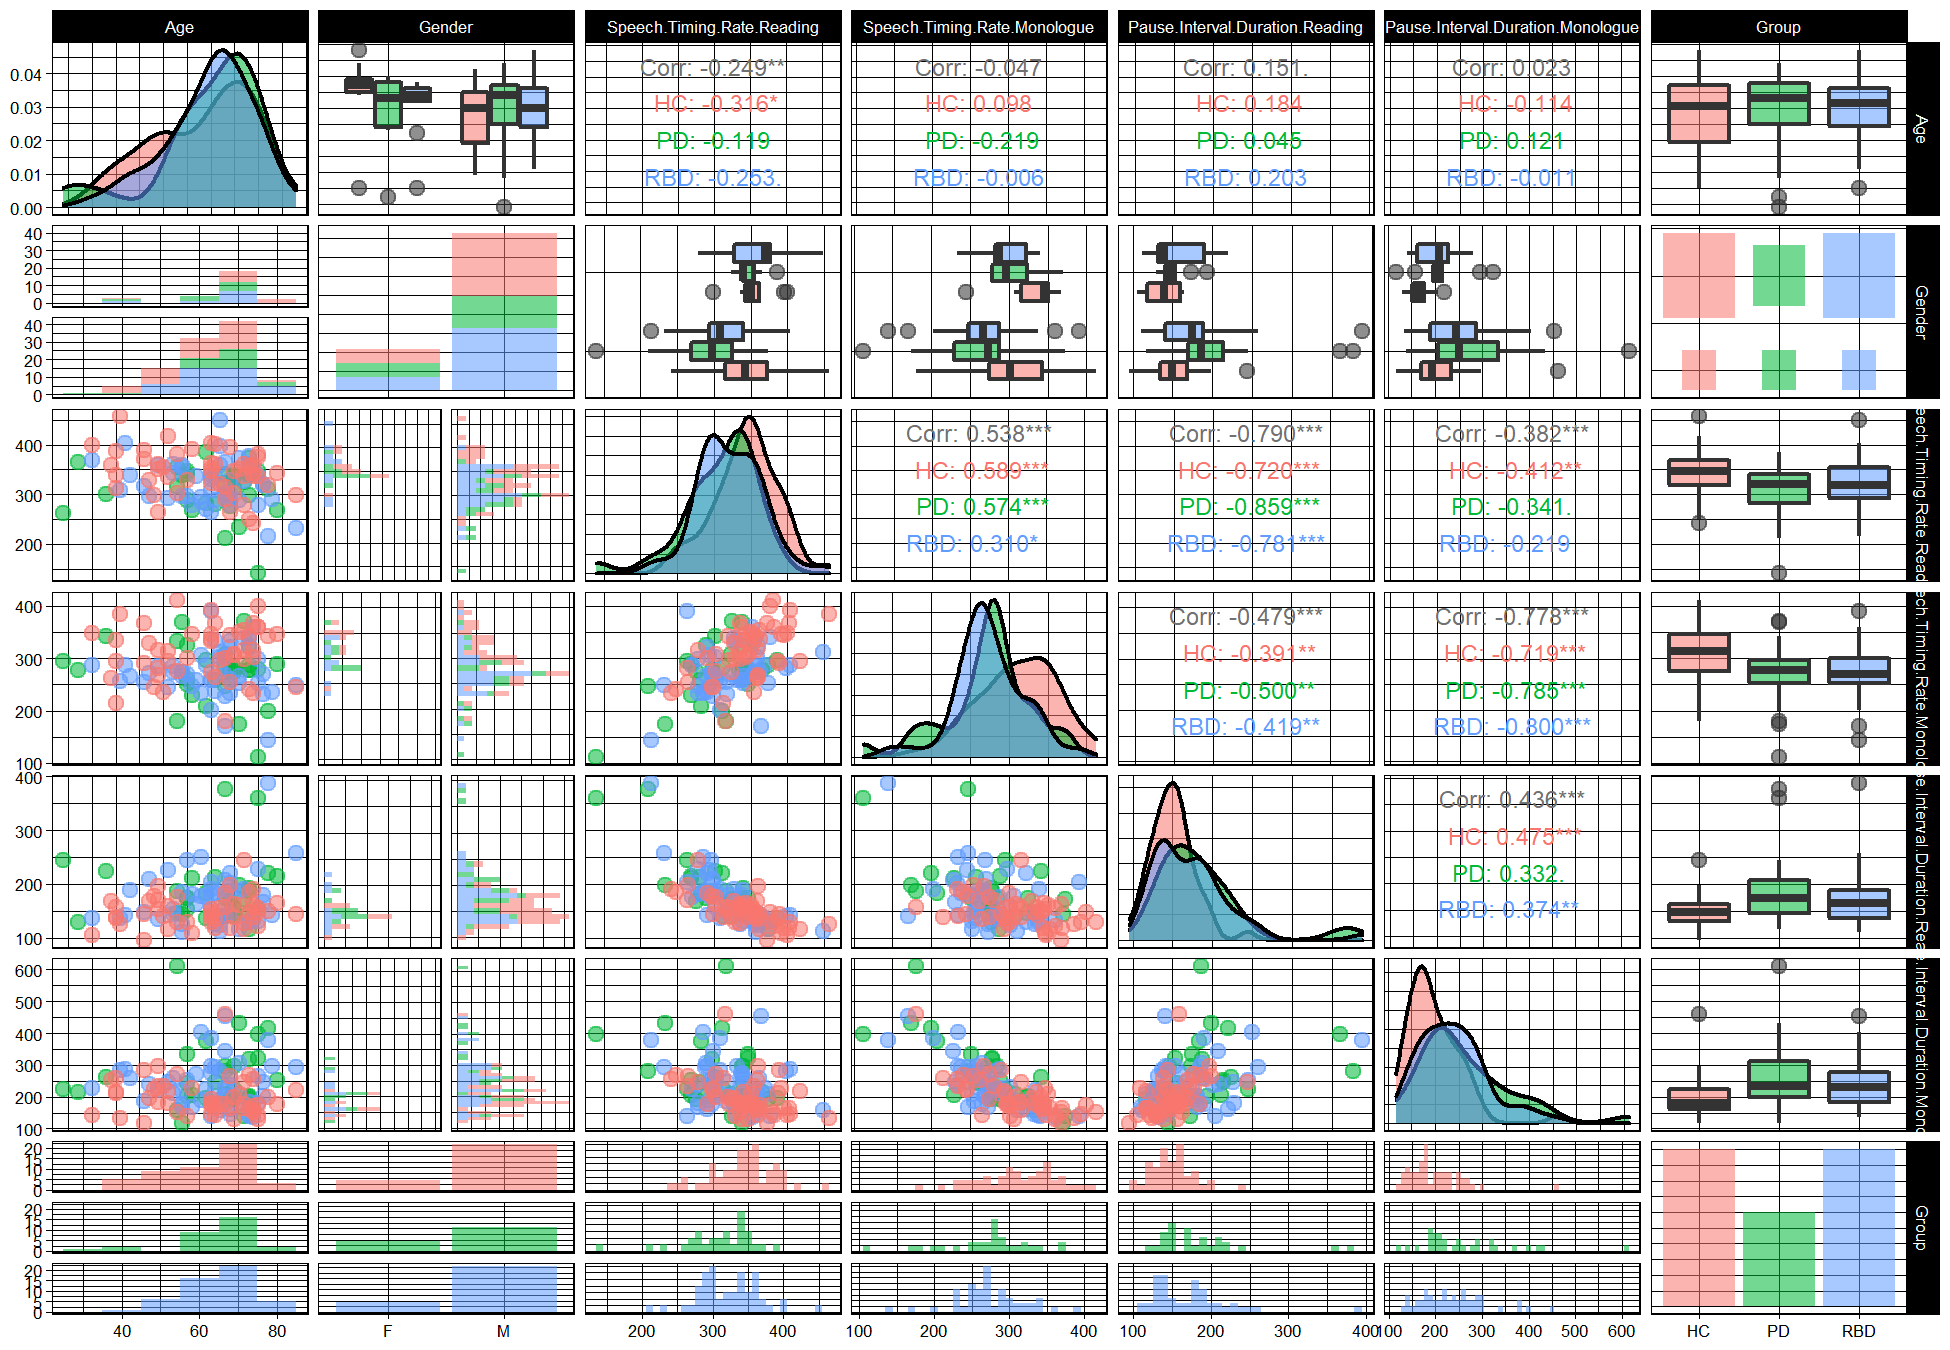
\includegraphics{dap_report_anja_probst_files/figure-latex/intial-ggpairs-plot-1} 

}

\caption{ }\label{fig:intial-ggpairs-plot}
\end{figure}

\begin{figure}

{\centering 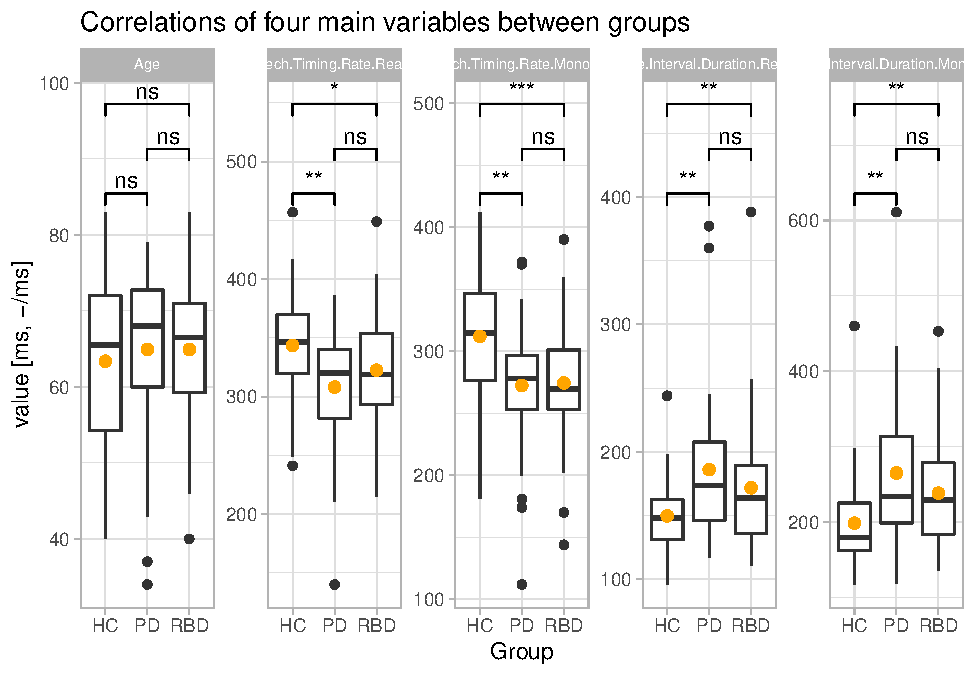
\includegraphics{dap_report_anja_probst_files/figure-latex/boxplots-and-correlations-1} 

}

\caption{ }\label{fig:boxplots-and-correlations}
\end{figure}
\clearpage

\hypertarget{data-analysis}{%
\section{Data Analysis}\label{data-analysis}}

\hypertarget{binomial-regression}{%
\subsection{Binomial Regression}\label{binomial-regression}}

Above, we have seen that there are almost no differences between the groups PD and RBD, so in a first step, we will limit our investigation to creating a binomial model predicting the group HC or PD. Indeed, the paper from which the data was extracted discusses the hard problem of differentiating PD from RBD, which might very well be impossible with generalised linear models. We will revisit this problem in the section Multinomial Regression.

\begin{figure}

{\centering 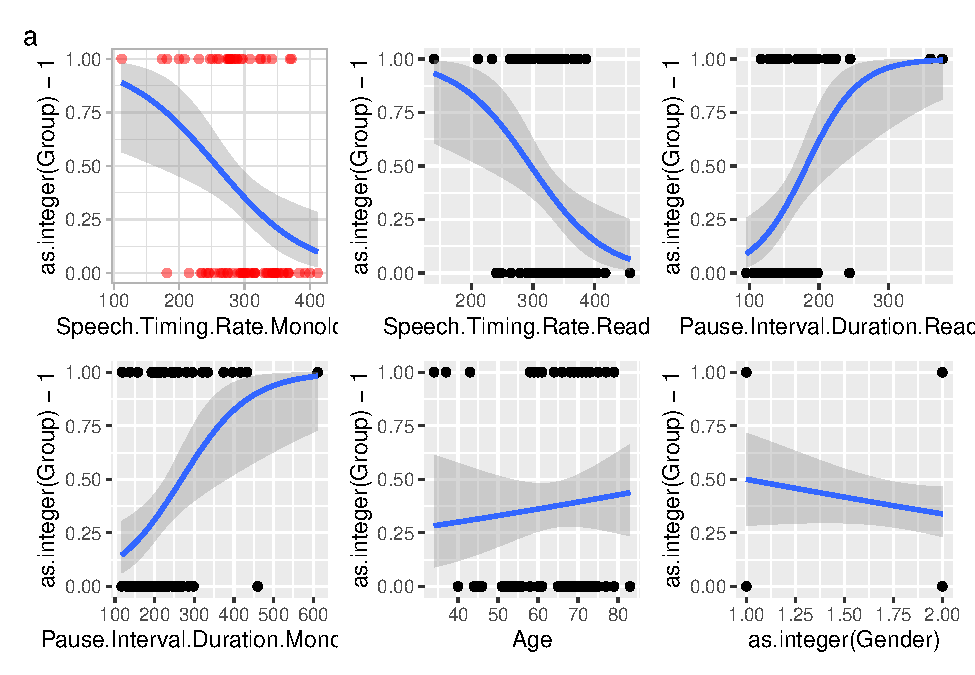
\includegraphics{dap_report_anja_probst_files/figure-latex/simple-linear-regression-1} 

}

\caption{ }\label{fig:simple-linear-regression}
\end{figure}

In a first step, a simple linear regression model based on a single predictor is built and visualized for each of the selected variables. As can be seen by visual inspection of the data points (red), none of the predictors is sufficient to predict the response variable (Group) on its own, given the respective overlap between the two groups. Hence, a series of multiple linear regression models have to be built and evaluated. As I would have to test 64 models (all possible combinations plus intercept only) to be certain to have found the best one, I chose to use the automated model selection function \texttt{dredge} from the R package \texttt{MuMIn}. Starting from the global binomial model \texttt{Group\ \textasciitilde{}\ .} as an input, \texttt{dredge} enumerates all possible models and evaluates them based on their AIC.

\begin{Shaded}
\begin{Highlighting}[]
\NormalTok{m.full }\OtherTok{\textless{}{-}} \FunctionTok{glm}\NormalTok{(}
  \AttributeTok{data=}\NormalTok{df.binom, Group }\SpecialCharTok{\textasciitilde{}}\NormalTok{ .,}
  \AttributeTok{family=}\NormalTok{binomial, }
  \AttributeTok{na.action =} \StringTok{"na.fail"}
\NormalTok{)}

\NormalTok{d }\OtherTok{\textless{}{-}} \FunctionTok{dredge}\NormalTok{(m.full, }\AttributeTok{rank =} \StringTok{"AIC"}\NormalTok{)}

\NormalTok{m.best.no.interactions }\OtherTok{=} \FunctionTok{get.models}\NormalTok{(d, }\DecValTok{1}\NormalTok{)[[}\DecValTok{1}\NormalTok{]]}
\end{Highlighting}
\end{Shaded}

\begin{table}[tbp]

\begin{center}
\begin{threeparttable}

\caption{\label{tab:table-best-model-dredge}A full regression table of the best model (selected using dredge) without interactions.}

\begin{tabular}{lllll}
\toprule
Predictor & \multicolumn{1}{c}{$b$} & \multicolumn{1}{c}{95\% CI} & \multicolumn{1}{c}{$z$} & \multicolumn{1}{c}{$p$}\\
\midrule
Intercept & -5.28 & $[-8.60$, $-2.53]$ & -3.42 & .001\\
GenderM & -1.76 & $[-3.15$, $-0.49]$ & -2.63 & .009\\
Pause Interval Duration Monologue & 0.01 & $[0.00$, $0.02]$ & 2.03 & .042\\
Pause Interval Duration Reading & 0.02 & $[0.01$, $0.05]$ & 2.39 & .017\\
\bottomrule
\end{tabular}

\end{threeparttable}
\end{center}

\end{table}

Looking at interactions \ldots{}

\begin{verbatim}
## 
## Call:
## glm(formula = Group ~ Pause.Interval.Duration.Reading:Pause.Interval.Duration.Monologue + 
##     Gender, family = binomial, data = df.binom)
## 
## Deviance Residuals: 
##     Min       1Q   Median       3Q      Max  
## -1.8600  -0.7777  -0.5119   0.9345   2.0621  
## 
## Coefficients:
##                                                                     Estimate
## (Intercept)                                                       -1.954e+00
## GenderM                                                           -1.650e+00
## Pause.Interval.Duration.Reading:Pause.Interval.Duration.Monologue  7.070e-05
##                                                                   Std. Error
## (Intercept)                                                        7.296e-01
## GenderM                                                            6.492e-01
## Pause.Interval.Duration.Reading:Pause.Interval.Duration.Monologue  1.976e-05
##                                                                   z value
## (Intercept)                                                        -2.678
## GenderM                                                            -2.541
## Pause.Interval.Duration.Reading:Pause.Interval.Duration.Monologue   3.577
##                                                                   Pr(>|z|)    
## (Intercept)                                                       0.007396 ** 
## GenderM                                                           0.011061 *  
## Pause.Interval.Duration.Reading:Pause.Interval.Duration.Monologue 0.000347 ***
## ---
## Signif. codes:  0 '***' 0.001 '**' 0.01 '*' 0.05 '.' 0.1 ' ' 1
## 
## (Dispersion parameter for binomial family taken to be 1)
## 
##     Null deviance: 105.850  on 79  degrees of freedom
## Residual deviance:  81.561  on 77  degrees of freedom
## AIC: 87.561
## 
## Number of Fisher Scoring iterations: 5
\end{verbatim}

\hypertarget{pca}{%
\subsubsection{PCA}\label{pca}}

As there has been significant correlation between the predictors in the ggpairs plot
as well as some extreme changes in coefficients when adding additional variables,
there exists the possbility of collinearity negatively affecting the models. Indeed,
we observe variance inflation factors of more than 2.5 between all experimental predictors.
This warrants and attempt at solving the potential collinearity issue.

\begin{verbatim}
##                               Age                            Gender 
##                          1.204231                          1.407117 
##        Speech.Timing.Rate.Reading      Speech.Timing.Rate.Monologue 
##                          3.073223                          2.916549 
##   Pause.Interval.Duration.Reading Pause.Interval.Duration.Monologue 
##                          2.599297                          2.652620
\end{verbatim}

\begin{verbatim}
## Importance of components:
##                           PC1    PC2     PC3     PC4
## Standard deviation     1.6786 0.8762 0.53096 0.36403
## Proportion of Variance 0.7045 0.1919 0.07048 0.03313
## Cumulative Proportion  0.7045 0.8964 0.96687 1.00000
\end{verbatim}

\begin{figure}

{\centering 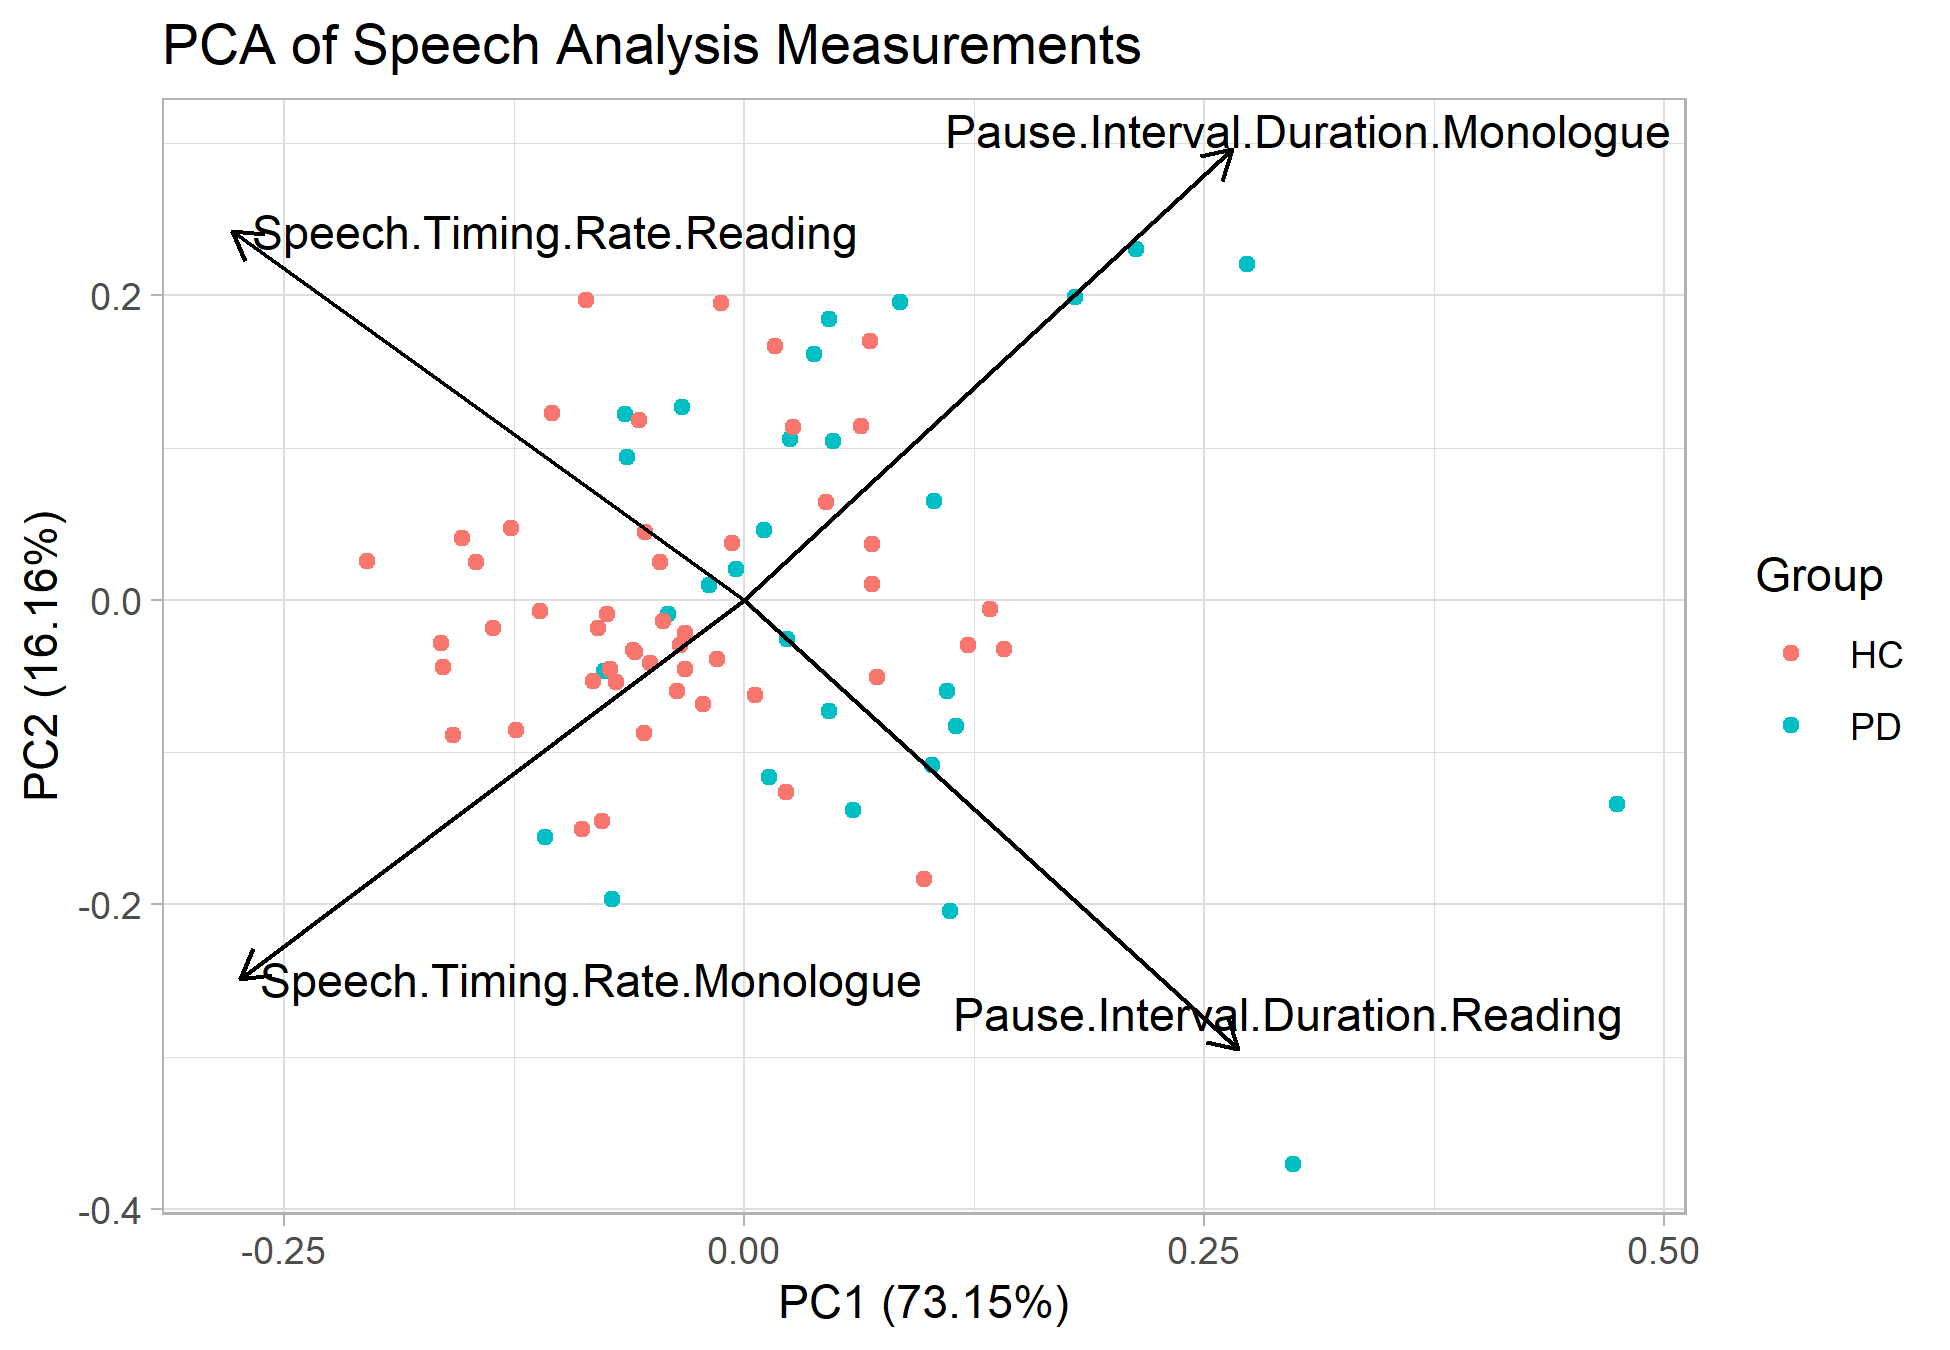
\includegraphics{dap_report_anja_probst_files/figure-latex/pca-loadings-1} 

}

\caption{ }\label{fig:pca-loadings}
\end{figure}

Running ggpairs shows, that there is no longer any correlation between the variables.

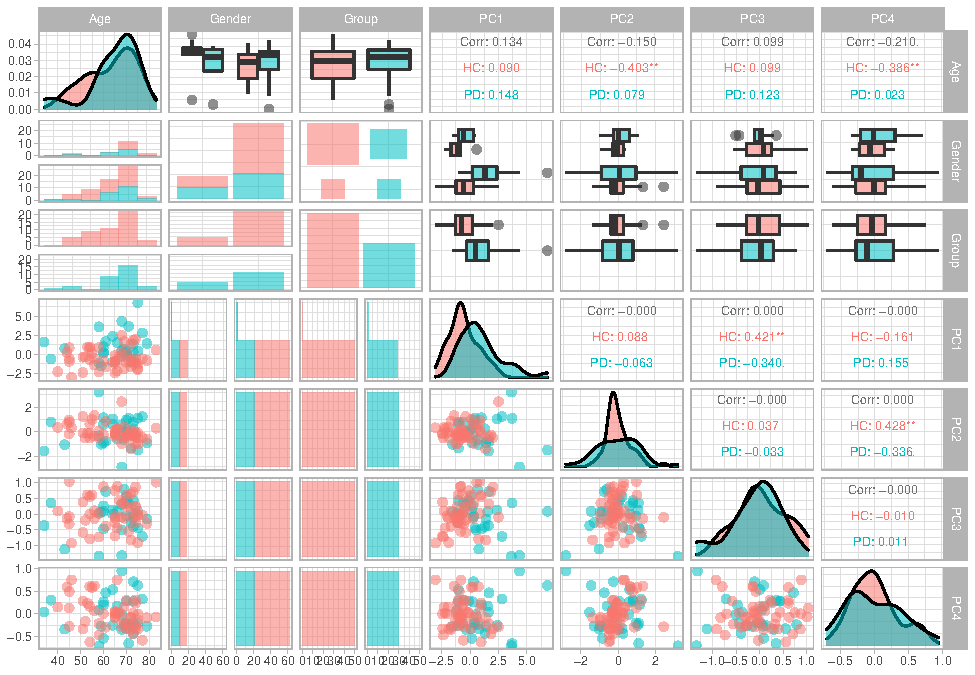
\includegraphics{dap_report_anja_probst_files/figure-latex/check for removal of correlations-1.pdf}

\begin{verbatim}
## 
## Call:
## glm(formula = Group ~ PC1 + Gender, family = "binomial", data = df.biom.pca.joined)
## 
## Deviance Residuals: 
##     Min       1Q   Median       3Q      Max  
## -1.7424  -0.7892  -0.4558   0.9875   2.0717  
## 
## Coefficients:
##             Estimate Std. Error z value Pr(>|z|)    
## (Intercept)   0.7417     0.5401   1.373 0.169734    
## PC1           0.9199     0.2456   3.746 0.000179 ***
## GenderM      -1.8062     0.6809  -2.653 0.007986 ** 
## ---
## Signif. codes:  0 '***' 0.001 '**' 0.01 '*' 0.05 '.' 0.1 ' ' 1
## 
## (Dispersion parameter for binomial family taken to be 1)
## 
##     Null deviance: 105.850  on 79  degrees of freedom
## Residual deviance:  81.454  on 77  degrees of freedom
## AIC: 87.454
## 
## Number of Fisher Scoring iterations: 5
\end{verbatim}

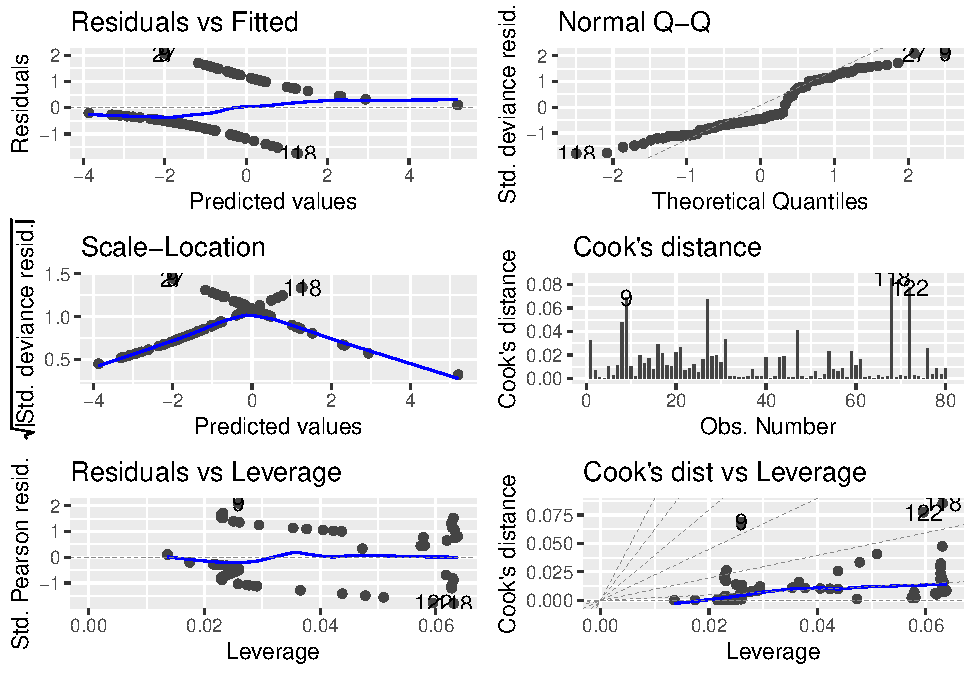
\includegraphics{dap_report_anja_probst_files/figure-latex/compare PCA-based model to best model from eval-1.pdf}

\begin{verbatim}
## Analysis of Deviance Table
## 
## Model 1: Group ~ PC1 + Gender
## Model 2: Group ~ Gender + Pause.Interval.Duration.Monologue + Pause.Interval.Duration.Reading + 
##     1
##   Resid. Df Resid. Dev Df Deviance Pr(>Chi)
## 1        77     81.454                     
## 2        76     80.274  1   1.1799   0.2774
\end{verbatim}

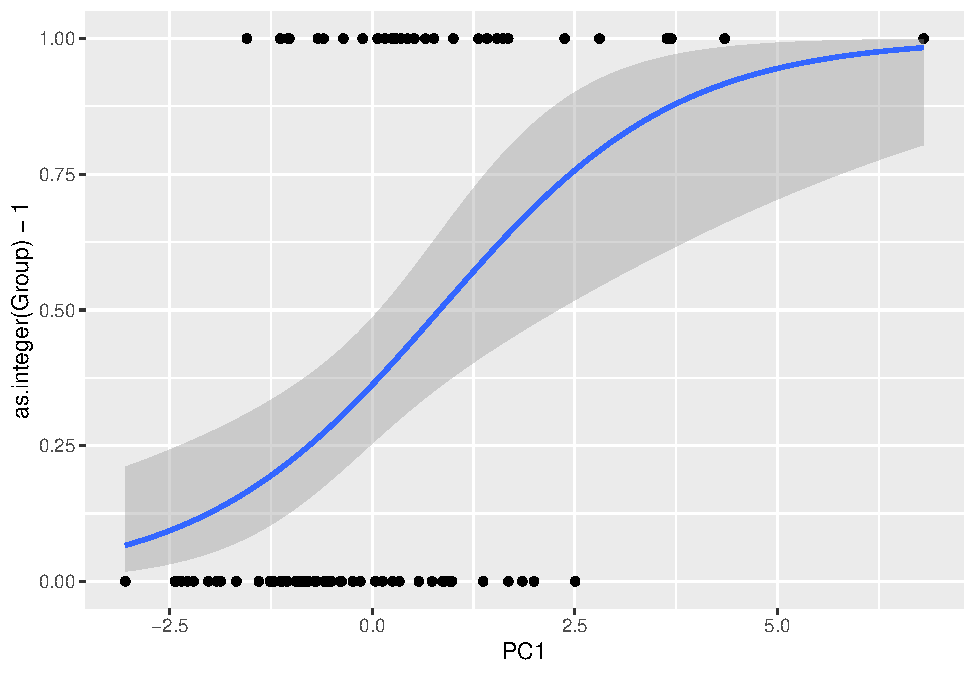
\includegraphics{dap_report_anja_probst_files/figure-latex/compare PCA-based model to best model from eval-2.pdf}

\hypertarget{multinomial-regression}{%
\subsection{Multinomial Regression}\label{multinomial-regression}}

To predict over all three groups (HC, PD, RBD), we have to use a more complex
multinomial model.

\begin{verbatim}
## # weights:  15 (8 variable)
## initial  value 99.973718 
## iter  10 value 86.144554
## iter  20 value 84.687289
## final  value 84.684738 
## converged
\end{verbatim}

\begin{verbatim}
##      
##       HC PD RBD
##   HC  28  1  10
##   PD   5  5   8
##   RBD  8  1  25
\end{verbatim}

\begin{verbatim}
## [1] 63.74
\end{verbatim}

\clearpage

\hypertarget{conclusion}{%
\section{Conclusion}\label{conclusion}}

\clearpage

\hypertarget{manual-model-plot}{%
\subsection{Manual Model Plot}\label{manual-model-plot}}

\clearpage

\hypertarget{references}{%
\section{References}\label{references}}

\begingroup
\setlength{\parindent}{-0.5in}
\setlength{\leftskip}{0.5in}

\hypertarget{refs}{}
\begin{CSLReferences}{0}{0}
\end{CSLReferences}

\endgroup


\end{document}
